\documentclass{standalone}
\usepackage{tikz}
\usetikzlibrary{patterns, positioning}
\usepackage[sfdefault]{ClearSans} %% option 'sfdefault' activates Clear Sans as the default text font
\usepackage[T1]{fontenc}

\begin{document}
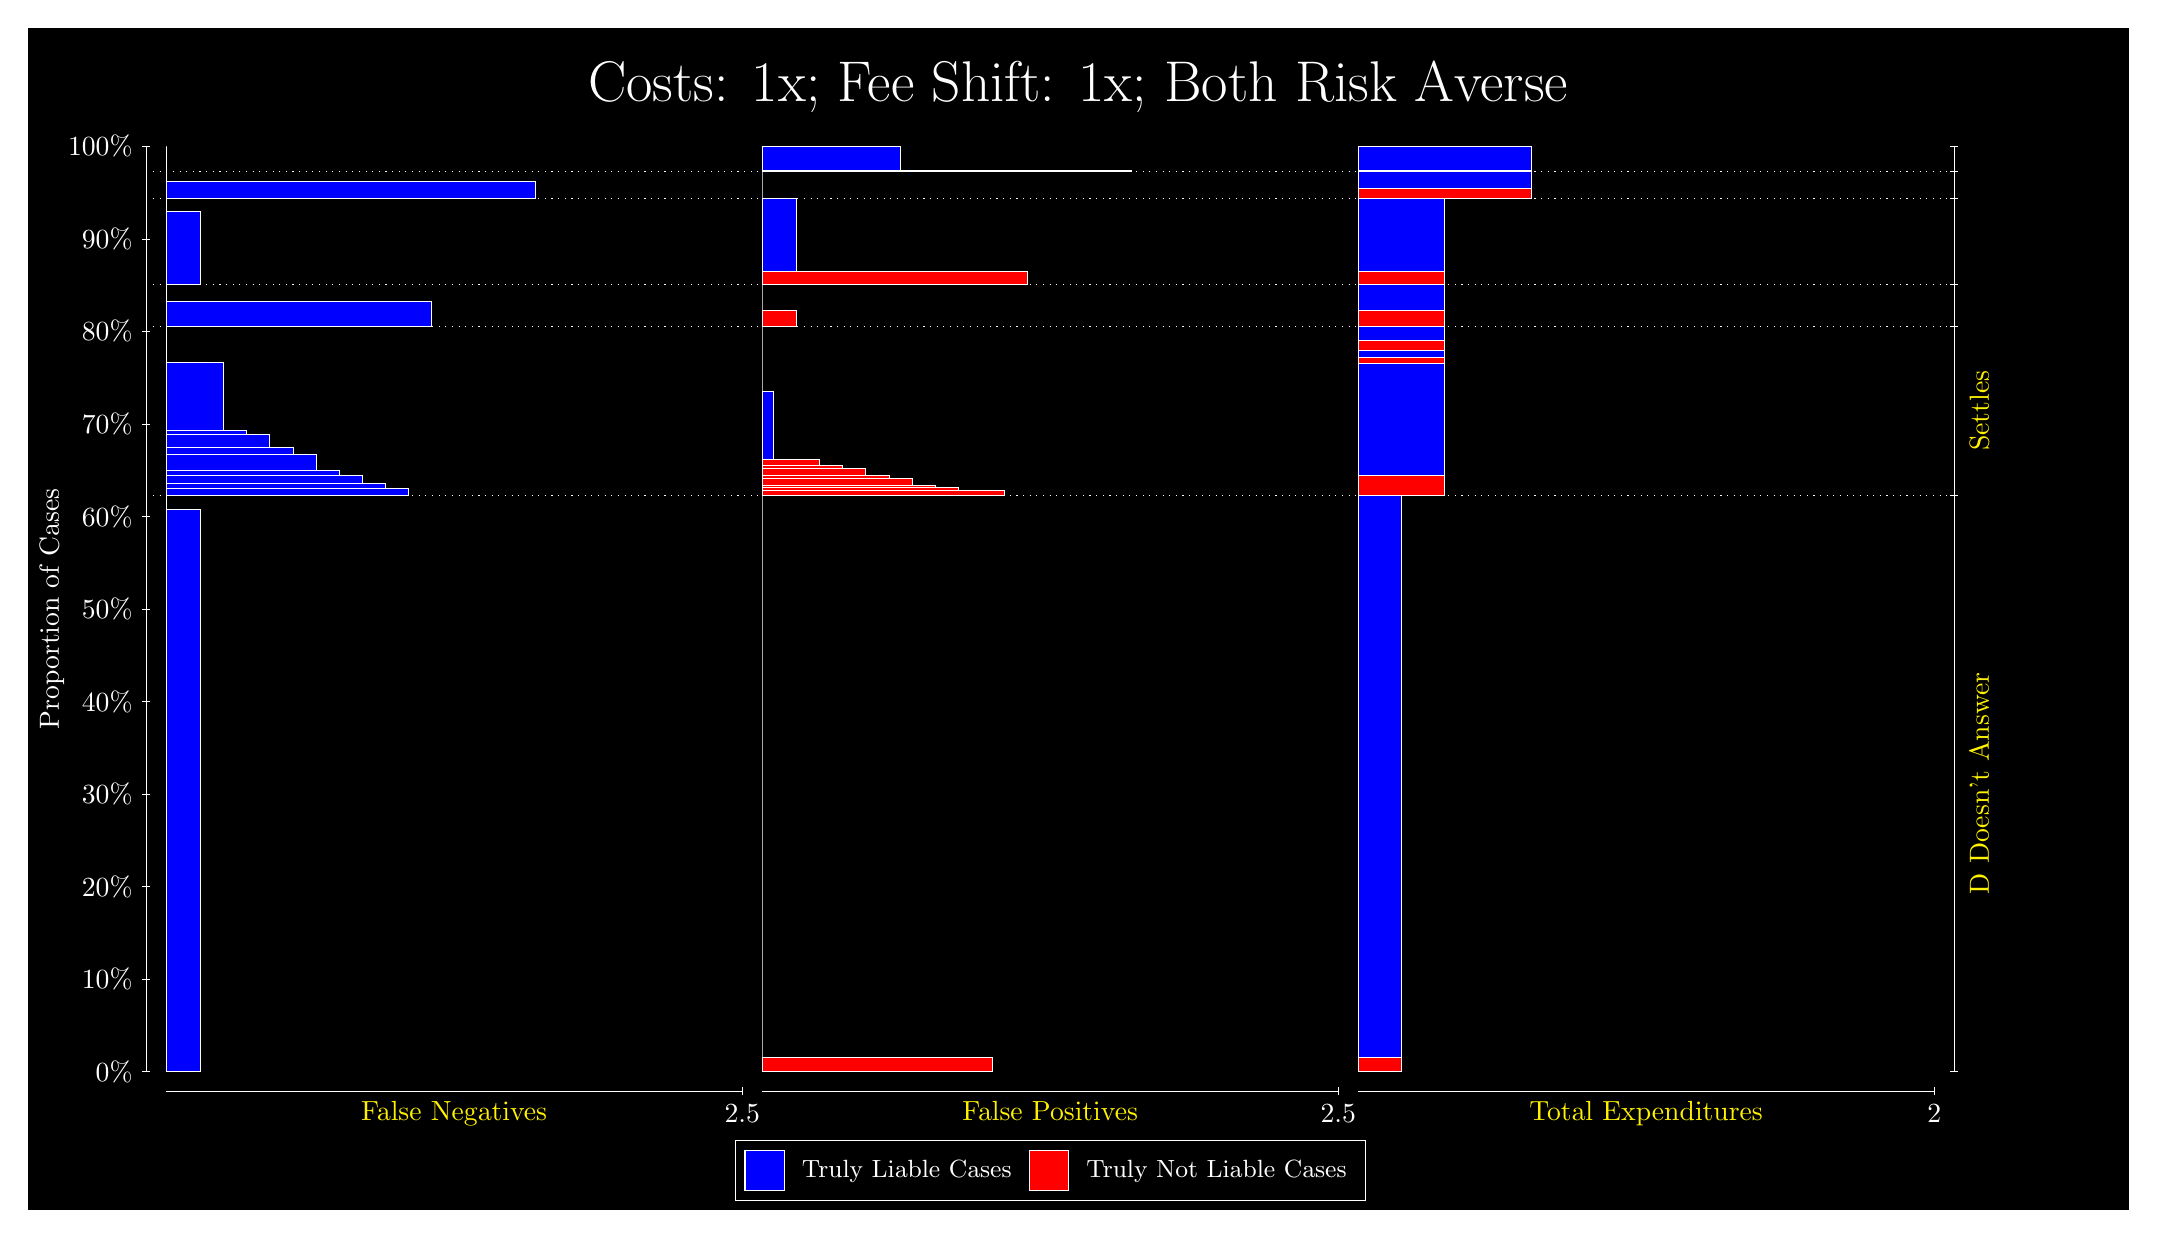
\begin{tikzpicture}
\draw[fill=black] (0,0) rectangle (26.667,15);
\draw[text=white] (0,13.5) rectangle (26.667,15) node[midway] {\huge Costs: 1x; Fee Shift: 1x; Both Risk Averse};
\draw[white, very thin] (1.5,1.75) -- (1.5,13.5);
\node[rotate=90, text=white, anchor=center] at (0.3, 7.625) {Proportion of Cases};
\draw[white, very thin] (1.45,1.75) -- (1.55,1.75);
\node[text=white, anchor=east] at (1.45, 1.75) {0\%};
\draw[white, very thin] (1.45,2.925) -- (1.55,2.925);
\node[text=white, anchor=east] at (1.45, 2.925) {10\%};
\draw[white, very thin] (1.45,4.1) -- (1.55,4.1);
\node[text=white, anchor=east] at (1.45, 4.1) {20\%};
\draw[white, very thin] (1.45,5.275) -- (1.55,5.275);
\node[text=white, anchor=east] at (1.45, 5.275) {30\%};
\draw[white, very thin] (1.45,6.45) -- (1.55,6.45);
\node[text=white, anchor=east] at (1.45, 6.45) {40\%};
\draw[white, very thin] (1.45,7.625) -- (1.55,7.625);
\node[text=white, anchor=east] at (1.45, 7.625) {50\%};
\draw[white, very thin] (1.45,8.8) -- (1.55,8.8);
\node[text=white, anchor=east] at (1.45, 8.8) {60\%};
\draw[white, very thin] (1.45,9.975) -- (1.55,9.975);
\node[text=white, anchor=east] at (1.45, 9.975) {70\%};
\draw[white, very thin] (1.45,11.15) -- (1.55,11.15);
\node[text=white, anchor=east] at (1.45, 11.15) {80\%};
\draw[white, very thin] (1.45,12.325) -- (1.55,12.325);
\node[text=white, anchor=east] at (1.45, 12.325) {90\%};
\draw[white, very thin] (1.45,13.5) -- (1.55,13.5);
\node[text=white, anchor=east] at (1.45, 13.5) {100\%};

\draw[white, very thin] (24.457,1.75) -- (24.457,13.5);
\draw[white, very thin] (24.407,1.75) -- (24.507,1.75);
\node[anchor=west] at (24.407, 1.75) {};
\draw[white, very thin] (24.407,9.0701) -- (24.507,9.0701);
\node[anchor=west] at (24.407, 9.0701) {};
\draw[white, very thin] (24.407,11.214) -- (24.507,11.214);
\node[anchor=west] at (24.407, 11.214) {};
\draw[white, very thin] (24.407,11.748) -- (24.507,11.748);
\node[anchor=west] at (24.407, 11.748) {};
\draw[white, very thin] (24.407,12.839) -- (24.507,12.839);
\node[anchor=west] at (24.407, 12.839) {};
\draw[white, very thin] (24.407,13.179) -- (24.507,13.179);
\node[anchor=west] at (24.407, 13.179) {};
\draw[white, very thin] (24.407,13.5) -- (24.507,13.5);
\node[anchor=west] at (24.407, 13.5) {};

\draw[white, very thin, fill=blue] (1.75,1.75) rectangle (2.1891,8.8849);
\draw[white, very thin, fill=red] (1.75,8.8849) rectangle (1.75,9.0701);
\draw[white, very thin, fill=blue] (1.75,9.0701) rectangle (4.8239,9.1632);
\draw[white, very thin, fill=blue] (1.75,9.1632) rectangle (4.5312,9.2154);
\draw[white, very thin, fill=blue] (1.75,9.2154) rectangle (4.2384,9.323);
\draw[white, very thin, fill=blue] (1.75,9.323) rectangle (3.9457,9.3891);
\draw[white, very thin, fill=blue] (1.75,9.3891) rectangle (3.6529,9.5871);
\draw[white, very thin, fill=blue] (1.75,9.5871) rectangle (3.3602,9.6752);
\draw[white, very thin, fill=blue] (1.75,9.6752) rectangle (3.0674,9.8384);
\draw[white, very thin, fill=blue] (1.75,9.8384) rectangle (2.7746,9.8909);
\draw[white, very thin, fill=blue] (1.75,9.8909) rectangle (2.4819,10.753);
\draw[white, very thin, fill=red] (1.75,10.753) rectangle (1.75,11.214);
\draw[white, very thin, fill=blue] (1.75,11.214) rectangle (5.1167,11.538);
\draw[white, very thin, fill=red] (1.75,11.538) rectangle (1.75,11.748);
\draw[white, very thin, fill=blue] (1.75,11.748) rectangle (2.1891,12.672);
\draw[white, very thin, fill=red] (1.75,12.672) rectangle (1.75,12.839);
\draw[white, very thin, fill=blue] (1.75,12.839) rectangle (6.4341,13.05);
\draw[white, very thin, fill=red] (1.75,13.05) rectangle (1.75,13.179);
\draw[white, very thin, fill=red] (1.75,13.179) rectangle (1.75,13.202);
\draw[white, very thin, fill=blue] (1.75,13.202) rectangle (1.75,13.5);
\draw[white, very thin, fill=red] (9.3189,1.75) rectangle (12.246,1.9352);
\draw[white, very thin, fill=blue] (9.3189,1.9352) rectangle (9.3189,9.0701);
\draw[white, very thin, fill=red] (9.3189,9.0701) rectangle (12.393,9.1258);
\draw[white, very thin, fill=red] (9.3189,9.1258) rectangle (12.1,9.1377);
\draw[white, very thin, fill=red] (9.3189,9.1377) rectangle (11.807,9.1743);
\draw[white, very thin, fill=red] (9.3189,9.1743) rectangle (11.515,9.1993);
\draw[white, very thin, fill=red] (9.3189,9.1993) rectangle (11.222,9.2877);
\draw[white, very thin, fill=red] (9.3189,9.2877) rectangle (10.929,9.3231);
\draw[white, very thin, fill=red] (9.3189,9.3231) rectangle (10.929,9.3281);
\draw[white, very thin, fill=red] (9.3189,9.3281) rectangle (10.636,9.4065);
\draw[white, very thin, fill=red] (9.3189,9.4065) rectangle (10.344,9.4492);
\draw[white, very thin, fill=red] (9.3189,9.4492) rectangle (10.051,9.5305);
\draw[white, very thin, fill=blue] (9.3189,9.5305) rectangle (9.4652,10.393);
\draw[white, very thin, fill=blue] (9.3189,10.393) rectangle (9.3189,11.214);
\draw[white, very thin, fill=red] (9.3189,11.214) rectangle (9.758,11.424);
\draw[white, very thin, fill=blue] (9.3189,11.424) rectangle (9.3189,11.748);
\draw[white, very thin, fill=red] (9.3189,11.748) rectangle (12.686,11.915);
\draw[white, very thin, fill=blue] (9.3189,11.915) rectangle (9.758,12.839);
\draw[white, very thin, fill=red] (9.3189,12.839) rectangle (9.3189,12.968);
\draw[white, very thin, fill=blue] (9.3189,12.968) rectangle (9.3189,13.179);
\draw[white, very thin, fill=red] (9.3189,13.179) rectangle (14.003,13.202);
\draw[white, very thin, fill=blue] (9.3189,13.202) rectangle (11.075,13.5);
\draw[white, very thin, fill=red] (16.888,1.75) rectangle (17.437,1.9352);
\draw[white, very thin, fill=blue] (16.888,1.9352) rectangle (17.437,9.0701);
\draw[white, very thin, fill=red] (16.888,9.0701) rectangle (17.986,9.3231);
\draw[white, very thin, fill=blue] (16.888,9.3231) rectangle (17.986,10.741);
\draw[white, very thin, fill=red] (16.888,10.741) rectangle (17.986,10.822);
\draw[white, very thin, fill=blue] (16.888,10.822) rectangle (17.986,10.915);
\draw[white, very thin, fill=red] (16.888,10.915) rectangle (17.986,11.041);
\draw[white, very thin, fill=blue] (16.888,11.041) rectangle (17.986,11.214);
\draw[white, very thin, fill=red] (16.888,11.214) rectangle (17.986,11.424);
\draw[white, very thin, fill=blue] (16.888,11.424) rectangle (17.986,11.748);
\draw[white, very thin, fill=red] (16.888,11.748) rectangle (17.986,11.915);
\draw[white, very thin, fill=blue] (16.888,11.915) rectangle (17.986,12.839);
\draw[white, very thin, fill=red] (16.888,12.839) rectangle (19.083,12.968);
\draw[white, very thin, fill=blue] (16.888,12.968) rectangle (19.083,13.179);
\draw[white, very thin, fill=red] (16.888,13.179) rectangle (19.083,13.202);
\draw[white, very thin, fill=blue] (16.888,13.202) rectangle (19.083,13.5);
\draw[white, dotted] (1.5,9.0701) -- (24.457,9.0701);
\draw[white, dotted] (1.5,11.214) -- (24.457,11.214);
\draw[white, dotted] (1.5,11.748) -- (24.457,11.748);
\draw[white, dotted] (1.5,12.839) -- (24.457,12.839);
\draw[white, dotted] (1.5,13.179) -- (24.457,13.179);
\draw[white, very thin] (1.75,1.5) -- (9.0689,1.5);
\node[text=yellow, anchor=north] at (5.4094, 1.5) {False Negatives};
\draw[white, very thin] (9.0689,1.45) -- (9.0689,1.55);
\node[text=white, anchor=north] at (9.0689, 1.45) {2.5};

\draw[white, very thin] (9.3189,1.5) -- (16.638,1.5);
\node[text=yellow, anchor=north] at (12.978, 1.5) {False Positives};
\draw[white, very thin] (16.638,1.45) -- (16.638,1.55);
\node[text=white, anchor=north] at (16.638, 1.45) {2.5};

\draw[white, very thin] (16.888,1.5) -- (24.207,1.5);
\node[text=yellow, anchor=north] at (20.547, 1.5) {Total Expenditures};
\draw[white, very thin] (24.207,1.45) -- (24.207,1.55);
\node[text=white, anchor=north] at (24.207, 1.45) {2};

\node[text=yellow, centered, rotate=90] at (24.777, 5.4101) {D Doesn't Answer};
\node[text=yellow, centered, rotate=90] at (24.777, 10.142) {Settles};





\draw (12.978300999999998,1.5) node[draw=none] (baseCoordinate) {};
\begin{scope}[align=center]
        \matrix[scale=0.5, draw=white, below=0.5cm of baseCoordinate, nodes={draw}, column sep=0.1cm]{
            \node[rectangle, draw, minimum width=0.5cm, minimum height=0.5cm, fill=blue] {}; &
            \node[draw=none, font=\small, text=white] (B) {Truly Liable Cases}; &
            \node[rectangle, draw, minimum width=0.5cm, minimum height=0.5cm, fill=red] {}; &
            \node[draw=none, font=\small, text=white] (B) {Truly Not Liable Cases}; \\
            };
\end{scope}

\end{tikzpicture}
\end{document}